% Author: PokMan Ho pok.ho19@imperial.ac.uk
% Script: nlls.tex
% Desc: nlls model fitting section
% Input: none
% Output: none
% Arguments: 0
% Date: Jan 2020

\documentclass[../note.tex]{subfiles} %% use packages & commands as this main file

\begin{document}

\section{Non-Linear Least Square (NLLS) Method}
When you data is not having linearity anywhere (e.g. growth, stress performance, functional response), you cannot use linear models (neither non-parametric nor parametric).  Hence if you want to explain your data with a published model, you can only try to tweak model parameters and make the model fit onto your data.  There are three ways (\href{https://datascienceplus.com/first-steps-with-non-linear-regression-in-r/}{NLLS}, \href{https://www.r-bloggers.com/fitting-a-model-by-maximum-likelihood/}{maximum likelihood} [ML] and \href{https://www.r-bloggers.com/bayesian-models-in-r-2/}{Bayesian Inference} [BI]).  This section will be only including methods taught in the ``Computational Methods in Ecology and Evolution" course at Silwood Park, original notes \href{https://nbviewer.jupyter.org/github/mhasoba/TheMulQuaBio/blob/master/notebooks/Appendix-ModelFitting.ipynb}{here}.

The logic is simple:
\begin{enumerate}
    \item Identify models of interest \& parameters you need to fit
    \item Try your best to estimate a value for each parameter (use recursive linear model and R$^2$ values to judge for you if needed)
    \item Use a distribution (either normal or uniform) to sample values around your guesstimated one
    \item Try to fit those sets of sampled parameter values (i.e. starting values) in your model on your data (run R function)
    \item Use AIC to extract the ``best guess" group among all the sampled parameter values
\end{enumerate}
This approach has some assumptions (of course, as always)
\begin{itemize}
    \item You try your best at guesstimating the values for sampling
    \item You did a good job in guesstimating values that the computer can tweak bit of the starting values, resulting to the overall best fit (i.e. global minimum of model fitting)
    \item if you use a normal distribution, it even mean that your guess is very close to the ``true value"
\end{itemize}
As you can see, these assumptions are based on ``you", because only human commit errors.  However computers are stubborn.  Once they have trials that converge to the same stable parameter value (i.e. local minimum), it assumes that convergence = best value.  As we know that local minimums can have values far from the global minimum, we have to be sure that our guess can let the computer end its job at the global minimum (modified visualization from original \href{http://www.ccl.net/cca/documents/molecular-modeling/fig22.gif}{source} below).
\begin{center}
    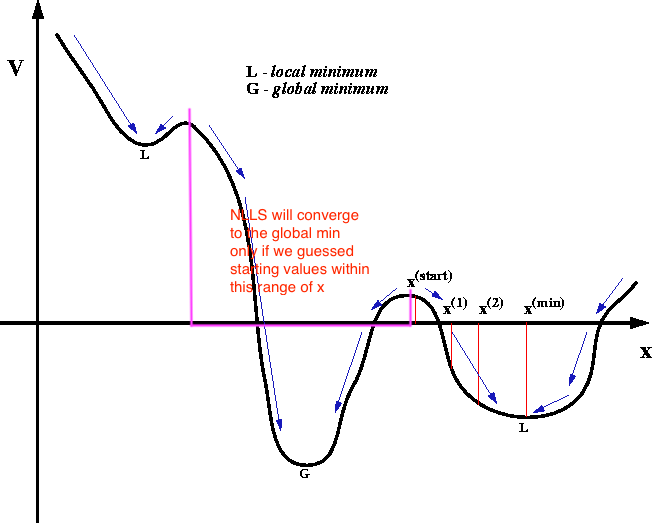
\includegraphics[width=.7\linewidth]{../graph/locMin.png}
\end{center}

\end{document}